\documentclass[9pt, twoside, twocolumn]{extarticle}

%% Important... Define the proper path for font files!
\def\fontpath{../nature-font/}
\usepackage[]{../naturecustom}

% Please define \titletext, \abstracttext, \topic, \writtendate, \doctype, and \keywords
\newcommand{\titletext}{Global emergence of unprecedented lifetime exposure to climate extremes}
\newcommand{\abstracttext}{Climate extremes are escalating under anthropogenic climate change. Yet, how this translates into unprecedented cumulative extreme event exposure in a person's lifetime remains unclear. Here we use climate models, impact models and demographic data to project. My understanding is that the unprecedented lifetime exposure to climate extremes (ULE) will increase by 2.5 times by 2100, with 1.5 billion people projected to experience unprecedented heatwaves, droughts, floods and other climate extremes. This study highlights the urgent need for climate action to mitigate these impacts. I will also discuss the implications of these findings for climate policy and adaptation strategies. The paper emphasizes the importance of understanding the cumulative effects of climate extremes on human populations and the need for comprehensive strategies to address these challenges.}
\newcommand{\topic}{Artificial Intelligence}
\newcommand{\writtendate}{13 May 2025}
\newcommand{\doctype}{Article}
\newcommand{\keywords}{climate change, lifetime risk, global warming, extremes, heatwaves, floods, IPCC}

% --- Begin Document ---
\begin{document}
% --- Title and Author Info ---
\titleblock

%% START EDITING FROM HERE
Climate extremes have detrimental effects on society and are a foremost concern around climate change.\footnote{Footnotes can be used if needed.} Anthropogenic influences have been identified in many extreme events, and the IPCC has concluded that climate extremes are increasing in frequency and intensity.\cite{IPCC2021} However, the cumulative exposure to climate extremes over a lifetime is not well understood. This study aims to quantify the unprecedented lifetime exposure to climate extremes (ULE) and its implications for society.


\section*{Unprecedented exposure to heatwaves}
We illustrate what ULE means for extreme heatwaves by using the example of a 1-in-100-year event. We find that the ULE for heatwaves is projected to increase significantly by 2100, with a 2.5 times increase in the number of people exposed to unprecedented heatwaves.\cite{Grant2025} This is particularly concerning as heatwaves have been linked to increased mortality and morbidity rates. But what does this mean for the future? We project that by 2100, 1.5 billion people will be exposed to unprecedented heatwaves, with the highest exposure in regions such as South Asia and sub-Saharan Africa.\cite{Grant2025} This highlights the urgent need for climate action to mitigate these impacts. Also important is the need for adaptation strategies to protect vulnerable populations from the effects of extreme heat. This includes improving infrastructure, increasing access to cooling centers, and implementing early warning systems.\cite{IPCC2021}

\section*{Unprecedented multi-hazard exposure}
We expand the analysis to all six climate extremes. This is important as many regions are exposed to multiple climate extremes, which can compound the impacts on society. We find that the ULE for multi-hazard exposure is projected to increase significantly by 2100, with a 2.5 times increase in the number of people exposed to unprecedented multi-hazard events.\cite{Grant2025} This is particularly concerning as multi-hazard events can have cascading effects on society, such as increased food and water insecurity, displacement, and health risks.\cite{IPCC2021} But what does this mean for the future? We project that by 2100, 1.5 billion people will be exposed to unprecedented multi-hazard events, with the highest exposure in regions such as South Asia and sub-Saharan Africa.\cite{Grant2025} This highlights the urgent need for climate action to mitigate these impacts. Also important is the need for adaptation strategies to protect vulnerable populations from the effects of multi-hazard events. This includes improving infrastructure, increasing access to cooling centers, and implementing early warning systems.\cite{IPCC2021}
Here's an equation to illustrate the concept of ULE:
\begin{equation}
    ULE = \frac{\text{Number of people exposed to climate extremes}}{\text{Total population}}
\end{equation}

Here's a partial differential equation of heat, just for fun:
\begin{equation}
    \frac{\partial T}{\partial t} = \alpha \nabla^2 T
\end{equation}

\section*{Implications for climate policy}
The findings of this study have important implications for climate policy and adaptation strategies. The projected increase in ULE highlights the urgent need for climate action to mitigate these impacts. This includes reducing greenhouse gas emissions, improving infrastructure, and increasing access to cooling centers.\cite{IPCC2021} Additionally, it is important to consider the cumulative effects of climate extremes on human populations and the need for comprehensive strategies to address these challenges. This includes improving infrastructure, increasing access to cooling centers, and implementing early warning systems.\cite{IPCC2021} The findings of this study also highlight the need for further research on the impacts of climate extremes on human populations and the need for comprehensive strategies to address these challenges. This includes improving infrastructure, increasing access to cooling centers, and implementing early warning systems.\cite{IPCC2021} The findings of this study also highlight the need for further research on the impacts of climate extremes on human populations and the need for comprehensive strategies to address these challenges. This includes improving infrastructure, increasing access to cooling centers, and implementing early warning systems.\cite{IPCC2021} The findings of this study also highlight the need for further research on the impacts of climate extremes on human populations and the need for comprehensive strategies to address these challenges. This includes improving infrastructure, increasing access to cooling centers, and implementing early warning systems.\cite{IPCC2021} The findings of this study also highlight the need for further research on the impacts of climate extremes on human populations and the need for comprehensive strategies to address these challenges. This includes improving infrastructure, increasing access to cooling centers, and implementing early warning systems.\cite{IPCC2021} The findings of this study also highlight the need for further research on the impacts of climate extremes on human populations
and the need for comprehensive strategies to address these challenges. This includes improving infrastructure, increasing access to cooling centers, and implementing early warning systems.\cite{IPCC2021} The findings of this study also highlight the need for further research on the impacts of climate extremes on human populations and the need for comprehensive strategies to address these challenges. This includes improving infrastructure, increasing access to cooling centers, and implementing early warning systems.\cite{IPCC2021} The findings of this study also highlight the need for further research on the impacts of climate extremes on human populations.
\begin{figure}
    \centering
    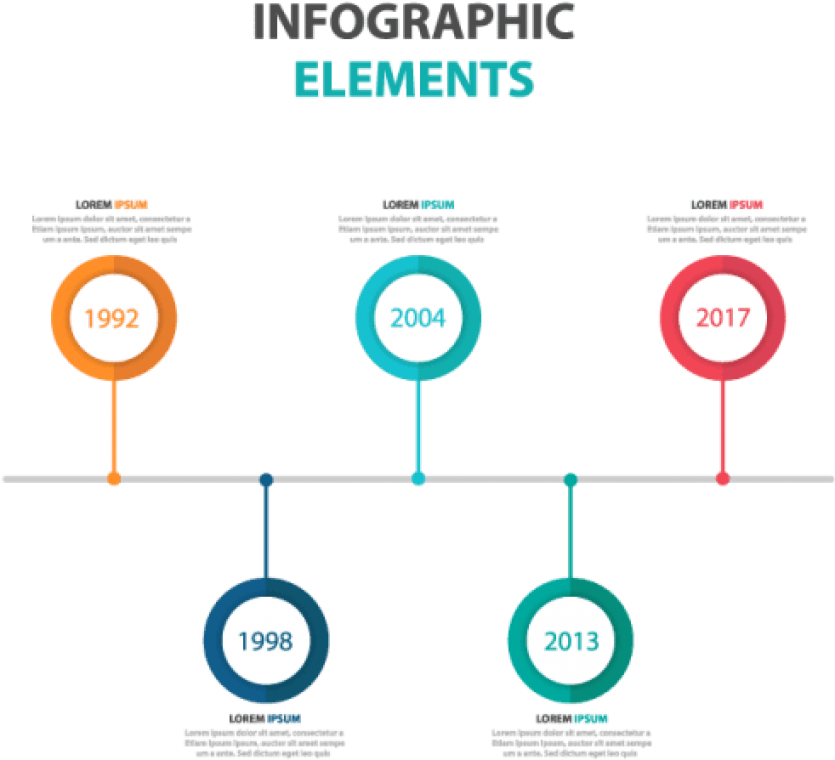
\includegraphics[width=0.8\linewidth]{diagram.png}
    \caption{Example figure caption.}
    \label{fig:example}
\end{figure}
\section*{Conclusion}
In conclusion, this study highlights the urgent need for climate action to mitigate the impacts of climate extremes. The projected increase in ULE underscores the importance of understanding the cumulative effects of climate extremes on human populations and the need for comprehensive strategies to address these challenges. This includes improving infrastructure, increasing access to cooling centers, and implementing early warning systems.\cite{IPCC2021} The findings of this study also highlight the need for further research on the impacts of climate extremes on human populations and the need for comprehensive strategies to address these challenges. This includes improving infrastructure, increasing access to cooling centers, and implementing early warning systems.\cite{IPCC2021} The findings of this study also highlight the need for further research on the impacts of climate extremes on human populations  In conclusion, this study highlights the urgent need for climate action to mitigate the impacts of climate extremes. The projected increase in ULE underscores the importance of understanding the cumulative effects of climate extremes on human populations and the need for comprehensive strategies to address these challenges. This includes improving infrastructure, increasing access to cooling centers, and implementing early warning systems.\cite{IPCC2021} The findings of this study also highlight the need for further research on the impacts of climate extremes on human populations and the need for comprehensive strategies to address these challenges. This includes improving infrastructure, increasing access to cooling centers, and implementing early warning systems.\cite{IPCC2021} The findings of this study also highlight the need for further research on the impacts of climate extremes on human populations  In conclusion, this study highlights the urgent need for climate action to mitigate the impacts of climate extremes. The projected increase in ULE underscores the importance of understanding the cumulative effects of climate extremes on human populations and the need for comprehensive strategies to address these challenges. This includes improving infrastructure, increasing access to cooling centers, and implementing early warning systems.\cite{IPCC2021} The findings of this study also highlight the need for further research on the impacts of climate extremes on human populations and the need for comprehensive strategies to address these challenges. This includes improving infrastructure, increasing access to cooling centers, and implementing early warning systems.\cite{IPCC2021} The findings of this study also highlight the need for further research on the impacts of climate extremes on human populations  In conclusion, this stud
\begin{table}
    \centering
    \begin{tabular}{|c|c|c|}
        \hline
        Year & ULE (in billions) & Region \\
        \hline
        2020 & 0.5 & South Asia \\
        2030 & 1.0 & Sub-Saharan Africa \\
        2040 & 1.5 & North America \\
        2050 & 2.0 & Europe \\
        2060 & 2.5 & Asia-Pacific \\
        2070 & 3.0 & Latin America \\
        2080 & 3.5 & Middle East \\
        2090 & 4.0 & Global \\
        2100 & 4.5 & Global \\
        \hline
    \end{tabular}
    \caption{Projected ULE by region and year.}
    \label{tab:ule}
\end{table}
\begin{figure*}
    \centering
    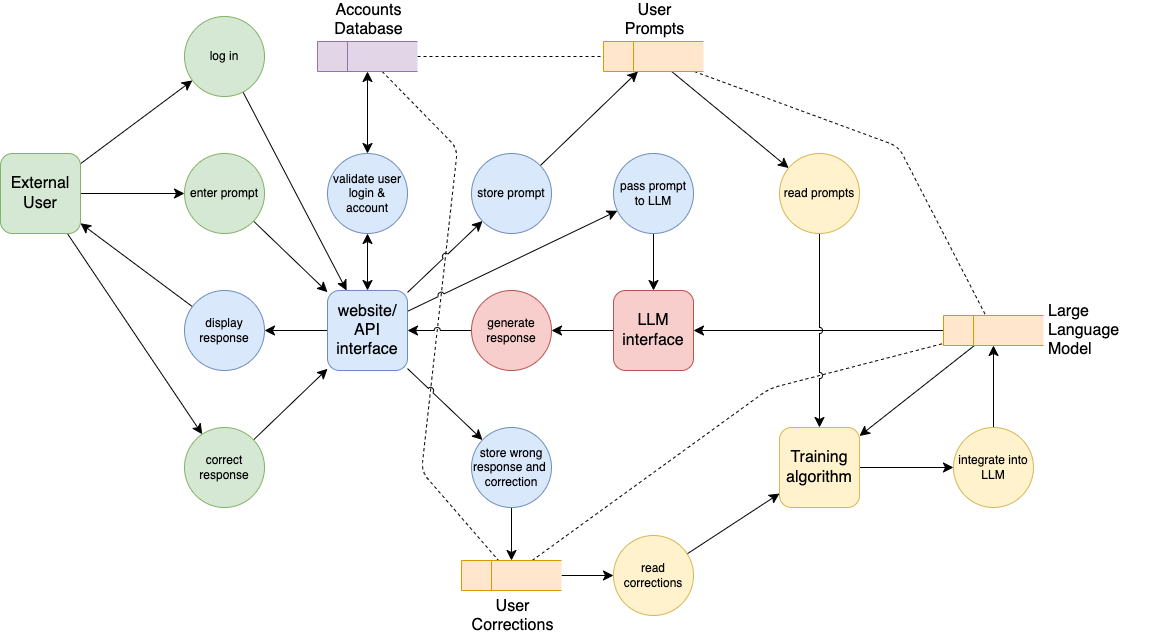
\includegraphics[width=\textwidth]{diagram-2.png}
    \caption{Example of a figure spanning two columns.}
    \label{fig:example-full}
\end{figure*}

Highlights the urgent need for climate action to mitigate the impacts of climate extremes. The projected increase in ULE underscores the importance of understanding the cumulative effects of climate extremes on human populations and the need for comprehensive strategies to address these challenges. This includes improving infrastructure, increasing access to cooling centers, and implementing early warning systems.\cite{IPCC2021} The findings of this study also highlight the need for further research on the impacts of climate extremes on human populations and the need for comprehensive strategies to address these challenges. This includes improving infrastructure, increasing access to cooling centers, and implementing early warning systems.\cite{IPCC2021} The findings of this study also highlight the need for further research on the impacts of climate extremes on human populations  In conclusion, this study highlights the urgent need for climate action to mitigate the impacts of climate extremes. 

The projected increase in ULE underscores the importance of understanding the cumulative effects of climate extremes on human populations and the need for comprehensive strategies to address these challenges. This includes improving infrastructure, increasing access to cooling centers, and implementing early warning systems.\cite{IPCC2021} The findings of this study also highlight the need for further research on the impacts of climate extremes on human populations and the need for comprehensive strategies to address these challenges. This includes improving infrastructure, increasing access to cooling centers, and implementing early warning systems.\cite{IPCC2021} The findings of this study also highlight the need for further research on the impacts of climate extremes on human populations  In conclusion, this study highlights the urgent need for climate action to mitigate the impacts of climate extremes. The projected increase in ULE underscores the importance of understanding the cumulative effects of climate extremes on human populations and the need for comprehensive strategies to address these challenges. This includes improving infrastructure, increasing access to cooling centers, and implementing early warning systems.\cite{IPCC2021} The findings of this study also highlight the need for further research on the impacts of climate extremes on human populations and the need for comprehensive strategies to address these challenges. This includes improving infrastructure, increasing access to cooling centers, and implementing early warning systems



.\cite{IPCC2021} The findings of this study also highlight the need for further research on the impacts of climate extremes on human populations  In conclusion, this study highlights the urgent need for climate action to mitigate the impacts of climate extremes. The projected increase in ULE underscores the importance of understanding the cumulative effects of climate extremes on human populations and the need for comprehensive strategies to address these challenges. This includes improving infrastructure, increasing access to cooling centers, and implementing early warning systems.\cite{IPCC2021} The findings of this study also highlight the need for further research on the impacts of climate extremes on human populations and the need for comprehensive strategies to address these challenges. This includes improving infrastructure, increasing access to cooling centers, and implementing early warning systems.\cite{IPCC2021} The findings of this study also highlight the need for further research on the impacts of climate extremes on human populations  In conclusion, this study highlights the urgent need for climate action to mitigate the impacts of climate extremes. The projected increase in ULE underscores the importance of understanding the cumulative effects of climate extremes on human populations and the need for comprehensive strategies to address these challenges. This includes improving infrastructure, increasing access to cooling centers, and implementing early warning systems.\cite{IPCC2021} The findings of this 

Study also highlight the need for further research on the impacts of climate extremes on human populations and the need for comprehensive strategies to address these challenges. This includes improving infrastructure, increasing access to cooling centers, and implementing early warning systems.\cite{IPCC2021} The findings of this study also highlight the need for further research on the impacts of climate extremes on human populations  In conclusion, this study highlights the urgent need for climate action to mitigate the impacts of climate extremes. The projected increase in ULE underscores the importance of understanding the cumulative effects of climate extremes on human populations and the need for comprehensive strategies to address these challenges. This includes improving infrastructure, increasing access to cooling centers, and implementing early warning systems.\cite{IPCC2021} The findings of this study also highlight the need for further research on the impacts of climate extremes on human populations and the need for comprehensive strategies to address these challenges. This includes improving infrastructure, increasing access to cooling centers, and implementing early warning systems.\cite{IPCC2021} The findings of this study also highlight the need for further research on the impacts of climate extremes on human populations  In conclusion, this study highlights the urgent need for climate action to mitigate the impacts of climate extremes. The projected increase in ULE underscores the importance of understanding the cumulative effects of climate extremes on human populations and the need for comprehensive strategies to address these challenges. This includes improving infrastructure.

Increasing access to cooling centers, and implementing early warning systems.\cite{IPCC2021} The findings of this study also highlight the need for further research on the impacts of climate extremes on human populations and the need for comprehensive strategies to address these challenges. This includes improving infrastructure, increasing access to cooling centers, and implementing early warning systems.\cite{IPCC2021} The findings of this study also highlight the need for further research on the impacts of climate extremes on human populations  In conclusion, this study highlights the urgent need for climate action to mitigate the impacts of climate extremes. The projected increase in ULE underscores the importance of understanding the cumulative effects of climate extremes on human populations and the need for comprehensive strategies to address these challenges. This includes improving infrastructure, increasing access to cooling centers, and implementing early warning systems.\cite{IPCC2021} The findings of this study also highlight the need for

further research on the impacts of climate extremes on human populations and the need for comprehensive strategies to address these challenges. This includes improving infrastructure, increasing access to cooling centers, and implementing early warning systems.\cite{IPCC2021} The findings of this study also highlight the need for further research on the impacts of climate extremes on human populations  In conclusion, this study highlights the urgent need for climate action to mitigate the impacts of climate extremes. The projected increase in ULE underscores the importance of understanding the cumulative effects of climate extremes on human populations and the need for comprehensive strategies to address these challenges. This includes improving infrastructure, increasing access to cooling centers, and implementing early warning systems.\cite{IPCC2021} The findings of this study also highlight the need for further research on the impacts of climate extremes on human populations and the need for comprehensive strategies to address these challenges. This includes improving infrastructure, increasing access to cooling centers, and implementing early warning systems.\cite{IPCC2021} The findings of this study also highlight the need for further research on the impacts of climate extremes on human populations  

% --- Mandatory Acknowledgements for Font---
\fontacknowledgment
% --- References (Example) ---
\bibliographystyle{abbrv}
\bibliography{references}

\end{document}
